\documentclass[english]{article}
\usepackage[T1]{fontenc}
\usepackage[utf8]{inputenc}
\usepackage{amsthm}
\usepackage{amsmath}
\usepackage{amsfonts}
\usepackage{listings}
\usepackage{babel}
\usepackage{tikz}

\newtheorem{thm}{\protect\theoremname}
\theoremstyle{definition}
\newtheorem*{example*}{\protect\examplename}
\theoremstyle{definition}
\newtheorem{example}[thm]{\protect\examplename}
\providecommand{\examplename}{Ejemplo}
\newtheorem*{defn*}{\protect\definitionname}
\providecommand{\definitionname}{Definición}
\newtheorem*{thm*}{\protect\theoremname}
\providecommand{\theoremname}{Teorema}


\begin{document}

\title{Control de concurrencia y recuperación en bases de datos}


\section{Transacciones y serializabilidad}

Construiremos un modelo para estudiar los problemas de concurrencia en bases
de datos. En este modelo, veremos a la base de datos como un conjunto de
ítems.

\begin{defn*}
Un \textbf{ítem} puede ser un atributo, una tupla o una relación entera; los
denominaremos con letras: $A$, $B$, $X$, $Y$.
\end{defn*}

\subsection{Transacciones}

\begin{defn*}
Llamaremos \textbf{transacción} a toda ejecución de un programa que accede a
la base de datos. El programa puede ejecutarse varias veces, y cada ejecución
del programa representa una nueva transacción $T_i$ ($i = 1, 2, \dots$).

La transacción es una sucesión de acciones (u operaciones), que representan
pasos atómicos. Estas acciones pueden ser:

\begin{itemize}
    \item Leer un ítem X ($r_i[X]$).
    \item Escribir un ítem X ($w_i[X]$).
    \item \emph{Abort} de la transacción $T_i$ ($a_i$).
    \item \emph{Commit} de la transacción $T_i$ ($c_i$).
\end{itemize}

Luego, una definición más precisa de transacción es la que sigue. $T_i$ es una
transacción si y sólo si:

$$T_i \subseteq \
    \{r_i[X], w_i[X], a_i, c_i: \
        X \mbox{ es un ítem, } i \in \mathbb{N}\}$$
\end{defn*}

El modelo en el que encaja la definición anterior es el llamado \emph{modelo
read-write} o \emph{modelo sin locking}. En él, las $T_i$ se ejecutan en forma
concurrente (entrelazada) y esto, veremos luego, puede llevar a la ocurrencia
de interferencias. Asimismo, pueden ocurrir fallas en medio de la ejecución de
la transacción. Trataremos esto último más adelante, cuando hablemos de
recuperación.

Dos problemas clásicos que pueden presentarse son conocidos como \emph{lost
update} y \emph{dirty read}.

\subsection{\emph{Lost update}}

El \emph{lost update} o actualización perdida ocurre cuando la actualización
hecha por una transacción $T_1$ se pierde a causa de la acción de otra
transacción $T_2$ sobre el mismo ítem; ambas transacciones leen el mismo valor
anterior del ítem y luego lo actualizan en forma sucesiva.

\begin{example}
Supongamos el programa $P$:
\begin{enumerate}
    \item $Read(A)$
    \item $A := A + 1$
    \item $Write(A)$
\end{enumerate}

La función $Read(A)$ copia el valor del ítem $A$ en disco a la variable local
$A$. De manera inversa, $Write(A)$ copia el valor de la variable local $A$ al
disco. $A := A + 1$ actualiza el valor de la variable local.

Supongamos ahora dos ejecuciones de $P$, $T_1$ y $T_2$, con el siguiente
entrelazamiento:

\vspace{10pt}

\begin{tabular}{ l l l }
  $T_1$         & $T_2$         & A (en disco)  \\
  \hline
  $Read(A)$     &               & 5             \\
                & $Read(A)$     & 5             \\
  $A := A + 1$  &               & 5             \\
                & $A := A + 1$  & 5             \\
                & $Write(A)$    & 6             \\
  $Write(A)$    &               & 6             \\
\end{tabular}

\vspace{10pt}

Notar que ocurre la siguiente secuencia:
\begin{enumerate}
    \item $T_1$ y $T_2$ leen el valor de $A$ desde el disco y lo almacenan en
        su variable local homónima.
    \item $T_1$ y $T_2$ actualizan el valor de su variable local $A$.
    \item $T_2$ escribe el valor actualizado de $A$ en disco, y luego lo hace
        $T_1$.
\end{enumerate}

Uno podría esperar que, luego de la ejecución de ambas transacciones, el valor
de $A$ en disco fuera incrementado dos veces. Sin embargo, al ejecutar las
transacciones concurrentemente, puede ocurrir que la actualización por parte
de una de las dos transacciones se pierda, como se observa en el ejemplo.
\end{example}

\subsection{\emph{Dirty read}}

Supongamos que tenemos dos transacciones $T_1$ y $T_2$. Supongamos también que
ambas operan sobre un mismo ítem $A$ en disco. Al ejecutarlas de manera
concurrente, podría darse la situación en que $T_1$ altere el valor del ítem
$A$ en disco, que $T_2$ tome ese valor alterado para operar y que luego $T_1$,
por alguna razón, falle.

Podríamos decidir que una característica deseable de las transacciones sea la
de ejecutarse siempre completamente o directamente no ejecutarse. En ese caso,
al enfrentarnos con la situación recién descripta, luego de abortar la
ejecución de $T_1$ (ya que incurrió en una falla), deberían volverse atrás
todas las operaciones que realizó esta transacción. El problema es que, para
entonces, $T_2$ ya comenzó a operar con el valor ``sucio'' de $A$. Este es el
problema del \emph{dirty read}.

Es buen momento para notar que, si se decide abortar $T_2$, porque leyó un
valor escrito por $T_1$ y esta abortó, entonces podría darse un caso de
\emph{aborts} en cascada: Podría existir una transacción $T_3$, que leyó un
valor escrito por $T_2$ y también deberá ser abortada, y podría existir $T_4$,
que leyó un valor escrito por $T_3$, y así sucesivamente. Más adelante
volveremos a hablar de este problema.

Veamos ahora, más en detalle, un ejemplo de \emph{dirty read}.

\begin{example}
Supongamos el programa $P_1$:
\begin{enumerate}
    \item $Read(A)$
    \item $A := A - 1$
    \item $Write(A)$
    \item $Read(B)$
    \item $B := B/A$
    \item $Write(B)$
\end{enumerate}

Y el programa $P_2$:
\begin{enumerate}
    \item $Read(A)$
    \item $A := A*2$
    \item $Write(A)$
\end{enumerate}

Supongamos entonces dos ejecuciones: Una de $P_1$ llamada $T_1$ y una de $P_2$
llamada $T_2$, con el siguiente entrelazamiento:

\vspace{10pt}

\begin{tabular}{ l l l l }
  $T_1$         & $T_2$         & A (en disco)  & B (en disco)  \\
  \hline
  $Read(A)$     &               & 1             & 2             \\
  $A := A - 1$  &               & 1             & 2             \\
  $Write(A)$    &               & 0             & 2             \\
                & $Read(A)$     & 0             & 2             \\
                & $A := A*2$    & 0             & 2             \\
  $Read(B)$     &               & 0             & 2             \\
                & $Write(A)$    & 0             & 2             \\
  $B := B/A$    &               & 0             & 2             \\
\end{tabular}

\vspace{10pt}

Los valores iniciales de $A$ y $B$ son 1 y 2, respectivamente.

Notar lo siguiente:
\begin{enumerate}
    \item $T_1$ actualiza el valor de $A$.
    \item $T_2$ lee el valor de $A$ almacenado por $T_1$.
    \item $T_1$ intenta realizar una división por cero, por lo que aborta.
        Luego se deberá volver el valor de $A$ al que tenía antes de
        ejecutarse $T_1$.
    \item El valor que leyó $T_2$ está ``sucio''; no es válido.
\end{enumerate}
\end{example}

\subsection{\emph{Non-repeatable read}}

El problema del \emph{non-repeatable read} se da cuando:
\begin{enumerate}
    \item Una transacción, $T_1$, lee el valor de un ítem $A$ del disco.
    \item Otra transacción, $T_2$, modifica el valor del mismo ítem en disco.
    \item $T_1$ lee el ítem $A$ de disco, nuevamente, y encuentra un valor
        distinto.
\end{enumerate}

El ejemplo queda como ejercicio para el lector. 

\subsection{\emph{Phantom read}}

El problema del \emph{phantom read} puede verse como un caso particular del
\emph{non-repeatable read}, siendo el origen de la lectura un \emph{query} y
siendo el ítem un conjunto de tuplas. En otras palabras, el
\emph{phantom read} ocurre cuando, en el avance de una transacción, dos
\emph{queries} idénticos son ejecutados y los conjuntos de tuplas resultantes
difieren.

\subsection{Propiedades ACID}

Las siguientes propiedades permiten garantizar que, dada una base de datos en
un estado consistente, luego de ejecutarse un número de transacciones, la base
de datos quede también en un estado consistente:

\begin{itemize}
    \item \textbf{A}tomicidad: Cada transacción se ejecuta por completo, o no
        se ejecuta.
    \item \textbf{C}onsistencia: La transacción en todos los casos debe llevar
        la base de datos de un estado consistente a otro consistente.
        
        La consistencia o no de la base de datos está dada por restricciones o
        expectativas que se tienen sobre ella. Por ejemplo, en una tabla de
        empleados, que el sueldo no sea negativo. Para que se cumpla esta
        propiedad, es necesario que los programas sean correctos.
    \item A\textbf{i}slamiento: Las transacciones se ejecutan sin
        interferencias.

        Es decir, debe parecer que, cuando se ejecuta una transacción, ninguna
        otra se está ejecutando al mismo tiempo.
    \item \textbf{D}urabilidad: Las actualizaciones a la base de datos hechas
        por una transacción, una vez que esta se completó, no deben perderse.
\end{itemize}

\subsection{Historias}

\begin{defn*}
Una \textbf{historia} es una secuencia de acciones tomadas por una o más
transacciones. En las historias, las acciones que efectúan las transacciones
tienen que estar en el mismo orden que se define en el programa de la
transacción, pero pueden entrelazarse acciones de distintas transacciones.

Es decir, podemos definir a las historias $H$ como una secuencia de $h_i$
tales que $h_i \in \{w_i[X], r_i[X], c_i, a_i\}$, con $X$ un ítem en la base
de datos (para los dos primeros casos) y tal que existe la transacción $T_i$,
y el orden de las acciones debe respetar al programa asociado a la
transacción.

Las historias pueden expresarse como secuencias de $h_i$ o en forma tabular.
\end{defn*}

\begin{example}
Una historia expresada en forma tabular, podría ser:

\begin{tabular}{ l l }
  $T_1$         & $T_2$     \\
  \hline
  $r[X]$        &           \\
                & $r[X]$    \\
  $w[X]$        &           \\
  $c$           &           \\
                & $w[Y]$    \\
                & $w[X]$    \\
                & $c$       \\
\end{tabular}
\end{example}

\subsubsection{Equivalencia de historias}

\begin{defn*}
Dos operaciones de dos transacciones distintas son \textbf{conflictivas} si
operan sobre el mismo ítem y al menos alguna de las dos es una escritura
($w_i$).
\end{defn*}

\begin{defn*}
Dos historias, $H$ y $H'$, son \textbf{equivalentes}, notado $H \equiv H'$ si:

\begin{enumerate}
    \item Involucran un mismo conjunto de transacciones.
    \item Las operaciones conflictivas tienen el mismo orden.
\end{enumerate}
\end{defn*}

\subsubsection{Historias seriales}

\begin{defn*}
La historia $H$ es \textbf{serial} si, para todo par de transacciones $T_i$ y
$T_j$ ($i \not= j$) involucradas en $H$, todas las operaciones de $T_i$
preceden a las de $T_j$ o viceversa, es decir, no hay entrelazamiento.
\end{defn*}

Las historias seriales, y las equivalentes a estas, son las que consideraremos
como correctas.

\subsubsection{Historias serializables}

\begin{defn*}
Una historia es \textbf{serializable} si es equivalente a una historia serial.
\end{defn*}

\subsubsection{Grafo de precedencia}

\begin{defn*}
Dada la historia $H$ sobre las transacciones $T_1, \dots, T_n$, un
\textbf{grafo de precedencia} $SG(H)$ es un grafo dirigido cuyos nodos son las
transacciones $T_i$ y existe un arco de $T_i$ a $T_j$ ($i \not= j$) toda vez
que alguna operación de $T_i$ precede y conflictúa con alguna operación de
$T_j$ en $H$.
\end{defn*}

\subsubsection{Teorema de serializabilidad}

\begin{thm}
Una historia $H$ es serializable si y sólo si su grafo de precedencia $SG(H)$
es acíclico. En ese caso, $H$ es equivalente a cualquier historia serial que
sea un ordenamiento topológico de $SG(H)$.
\end{thm}

Un algoritmo para obtener un orden topológico es el siguiente:

\begin{enumerate}
    \item Tomar uno de los nodos en el grafo a los cuales no llegan arcos.
    \item Agregar el nodo a la secuencia que representa el orden topológico.
    \item Quitar el nodo junto con todos los arcos que salen de él del grafo.
    \item Volver a 1.
\end{enumerate}

El algoritmo termina cuando ya no quedan nodos en el grafo.

\section{\emph{Locking}}

\begin{defn*}
Un \textbf{lock} es un privilegio de acceso a un ítem de la base de datos.
\end{defn*}

Decimos que una transacción ``obtiene un \emph{lock}'' sobre un ítem.

\subsection{\emph{Locking} binario}

En el modelo de \emph{locking} binario, existen dos estados posibles para los
ítems:

\begin{itemize}
    \item \textbf{Locked}. En programas, usamos $Lock(X)$ y en las historias
        $l_i[X]$.
    \item \textbf{Unlocked}. Usamos $Unlock(X)$ y $u_i[X]$.
\end{itemize}

El \emph{lock} binario siempre fuerza exclusión mutua sobre un ítem entre
transacciones, es decir, si una transacción adquirió el \emph{lock} sobre un
ítem, esta es la única que puede acceder al ítem hasta tanto no libere el
\emph{lock} sobre este.

\subsection{\emph{Locking} ternario}

Este modelo permite mayor concurrencia que el binario. En él, existen tres
estados posibles para los ítems:

\begin{itemize}
    \item \textbf{Read locked}. En programas, usamos $RLock(X)$ y en las
        historias $rl_i[X]$.
    \item \textbf{Write locked}. Usamos $WLock(X)$ y $wl_i[X]$.
    \item \textbf{Unlocked}. Usamos $ULock(X)$ y $ul_i[X]$ o $u_i[X]$.
\end{itemize}

El \emph{read lock} es un \emph{lock} compartido, mientras que el
\emph{write lock} es un \emph{lock} exclusivo. En otras palabras, si una
transacción tiene tomado un \emph{read lock} sobre un ítem, otras
transacciones también pueden obtener un \emph{read lock} sobre ese mismo ítem.
Sin embargo, el \emph{write lock} funciona de manera exclusiva, como en el
caso del \emph{locking} binario.

Puede darse el caso en que una transacción que tiene un \emph{read lock} sobre
un ítem quiera tomar un \emph{write lock} sobre él. En ese caso, ocurre una
conversión del primer \emph{lock} al último (\emph{lock conversion}), sólo si
no hay ninguna otra transacción que tenga tomado un \emph{read lock} sobre el
ítem.

\subsection{Modelo basado en \emph{Locking}}

En el modelo basado en \emph{locking}, una transacción es vista como una
secuencia de \emph{locks} y \emph{unlocks}. Las operaciones de escritura o
lectura son abstraídas.

\subsection{Reglas de legalidad de \emph{locking}}

Una historia es legal si:

\begin{itemize}
    \item Una transacción no puede leer ni escribir un ítem hasta tanto no
        haya obtenido un \emph{lock} sobre este.
    \item Si una transacción precisa un \emph{lock} sobre un ítem y
        otra transacción ya ha obtenido un \emph{lock} sobre ese ítem, de
        manera que ambos \emph{locks} conflictúan, entonces la primera debe
        esperar hasta que la última libere el \emph{lock}.
\end{itemize}
        
\subsubsection{Grafo de precedencia}

El grafo de precedencia en el modelo basado en \emph{locking} se define igual
que como lo hicimos anteriormente, sólo que entendemos el conflicto según las
reglas del \emph{locking}:

\begin{itemize}
    \item Para el caso del \emph{locking} binario, hay un conflicto si una
        transacción obtiene un \emph{lock} sobre un ítem y luego otra hace lo
        mismo sobre el mismo ítem.
    \item Para el caso del \emph{locking} ternario, hay un conflicto si una
        transacción obtiene un \emph{lock} sobre un ítem (sea de lectura o
        escritura) y luego otra obtiene un \emph{lock} (sea de lectura o
        escritura) sobre el mismo ítem, con la sola excepción de que no se
        produce un conflicto si ambos \emph{locks} son de lectura.
\end{itemize}


\begin{example}
Supongamos la siguiente historia, para el modelo de \emph{locking} binario:
$H = l_2[A], u_2[A], l_3[A], u_3[A], l_1[B], u_1[B], l_2[B], u_2[B]$.

Observar que $H$ es legal. Para ver si es serializable, podemos construir su
grafo de precedencia $SG(H)$: 

\vspace{10pt}

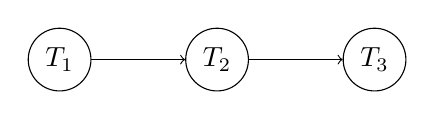
\begin{tikzpicture}
    [every node/.style={circle,draw=black}]
    \node (t1) at (0,0) {$T_1$};
    \node (t2) at (2,0) {$T_2$};
    \node (t3) at (4,0) {$T_3$};

    \foreach \from/\to in
        {t1/t2, t2/t3}
    \draw [->] (\from) -- (\to);

\end{tikzpicture}

Observamos que sí es serializable (el grafo no tiene ciclos) y es equivalente
a la historia serial $H_s = T_1, T_2, T_3$.
\end{example}

\begin{example}
Ahora supongamos la siguiente historia, para el modelo de \emph{locking}
ternario:

\vspace{10pt}

\begin{tabular}{ l l l l }
  $T_1$         & $T_2$     & $T_3$     & $T_4$     \\
  \hline
                &           & $wl_3[A]$ &           \\
                &           &           & $rl_4[B]$ \\
                &           & $ul_3[A]$ &           \\
  $rl_1[A]$     &           &           &           \\
                &           &           & $ul_4[B]$ \\
                &           & $wl_3[B]$ &           \\
                & $rl_2[A]$ &           &           \\
                &           & $ul_3[B]$ &           \\
  $wl_1[B]$     &           &           &           \\
                & $ul_2[A]$ &           &           \\
  $ul_1[A]$     &           &           &           \\
                &           &           & $wl_4[A]$ \\
  $ul_1[B]$     &           &           &           \\
                & $rl_2[B]$ &           &           \\
                &           &           & $ul_4[A]$ \\
                & $ul_2[B]$ &           &           \\
  \hline
\end{tabular}

\vspace{10pt}

Observar que esta historia es legal. Sin embargo, al construir su grafo de
precedencia, observamos que este tiene ciclos, lo que nos indica que la
historia no es serializable.
\end{example}


\newpage

\section{Apuntes para el parcial}

\subsection{\emph{Locking}}

\begin{defn*}
Una transacción $T$ es \textbf{2PL} (\emph{two phase locking}) si todos los
\emph{locks} preceden al primer \emph{unlock}.
\end{defn*}

\begin{thm*}
Sea un conjunto de transacciones. Si toda transacción en el conjunto es 2PL,
entonces toda historia legal sobre ese conjunto es serializable.
\end{thm*}

\subsection{Recuperabilidad}

\begin{defn*}
Definimos el operador $<$, para las acciones, del siguiente modo:
$a < b$ si y sólo si la acción $a$ precede a la acción $b$ en el orden de
ejecución.
\end{defn*}

\begin{defn*}
Sean las transacciones $T_i$ y $T_j$. Decimos que $T_i$ \textbf{lee de} $T_j$
en una historia $H$, si se da algún caso en que $T_j$ es la última transacción
que escribió en $X$, y no abortó, al momento en que $T_i$ lee de $X$.

%\begin{enumerate}
%    \item $\exists w_j[X], r_i[X] \in H$ y $w_j[X] < r_i[X]$
%    \item $\not\exists a_j \in H: a_j < r_i[X]$
%\end{enumerate}
\end{defn*}

\subsubsection{Clasificación de historias según recuperabilidad}
\begin{itemize}
	\item \textbf{RC (Recuperable):} Si siempre que una transacción lee de
        otra, esta última hizo \emph{commit} antes que la primera lo haga.
    \item \textbf{ACA (Evita aborts en cascada)}: Si siempre que una
        transacción lee de otra, esta última hizo \emph{commit} antes de la
        lectura.
    \item \textbf{ST (Estricta)}: Si siempre, al momento en que una
        transacción lee o escribe un ítem, la transacción que escribió antes
        sobre ese ítem ya hizo \emph{abort} o bien \emph{commit}.
\end{itemize}

\begin{thm*}
Se cumple que:

$$ ST \subset ACA \subset RC$$
\end{thm*}

\subsubsection{Recuperabilidad y serializabilidad}

Recuperabilidad y serializabilidad son conceptos ortogonales. Hay historias
serializables en no RC, RC, ACA y ST.

Notar que las historias seriales son SR (trivialmente) y ST.

\begin{defn*}
Una transacción $T$ es \textbf{2PL estricto} si es 2PL y, además, no libera
ningún \emph{lock} exclusivo (\emph{write lock}) hasta después de haber hecho
\emph{commit} o \emph{abort}.
\end{defn*}

\begin{thm*}
Toda historia que cumple 2PL estricto (sus transacciones cumplen 2PL estricto)
es SR, en cuanto serializabilidad, y ST, en cuanto a recuperabilidad.
\end{thm*}


\end{document}
